\documentclass[twocolumn]{article}[ht]

\usepackage[utf8]{inputenc}
\usepackage{graphicx} 
\usepackage{geometry} 
\usepackage{amsmath}
\usepackage{cite}
\geometry{
  left=17mm,
  right=17mm,
  top=15mm,
  bottom=15mm
}

\title{Solving one‐dimensional time independent Schrödinger equation by the localized Green’s function method}
\author{Hoang Nguyen \\ \textit{Universite de Bourgogne}}
\date{\today}

\begin{document}

\maketitle

\section{Introduction}
This report explores the one-dimensional time-independent Schrödinger equation using localized Green's functions for electron scattering at quantum junctions. It analyzes unbiased and biased junctions, studying spectral responses, transmission, reflection, probability densities, and potential profiles, while emphasizing phenomena like resonant tunneling and Negative Differential Resistance (NDR).
\section{Methods and Results}
\subsection{Constant Background}

This section investigates a reference system characterized by a constant potential background, defined as \(U_0 = 0 \, \text{eV} \, \forall x\). The associated Green's function for this system is described by the following equation:
\begin{equation}
    G_0(x, x'; k) = \frac{e^{ik |x - x'|}}{2ik}
\end{equation}

Given the conditions of the potential profile as below, the barriers are plotted.
\begin{equation}
    U(x') =
    \begin{cases}
        0.2 \text{eV}; & \forall x\ \in [0 \text{\AA}, 15 \text{\AA}] \\
        0.2 \text{eV}; & \forall x\ \in [65 \text{\AA}, 80 \text{\AA}] \\
        0 & \text{elsewhere}
    \end{cases}
\end{equation}

\begin{figure}[ht]
    \centering
    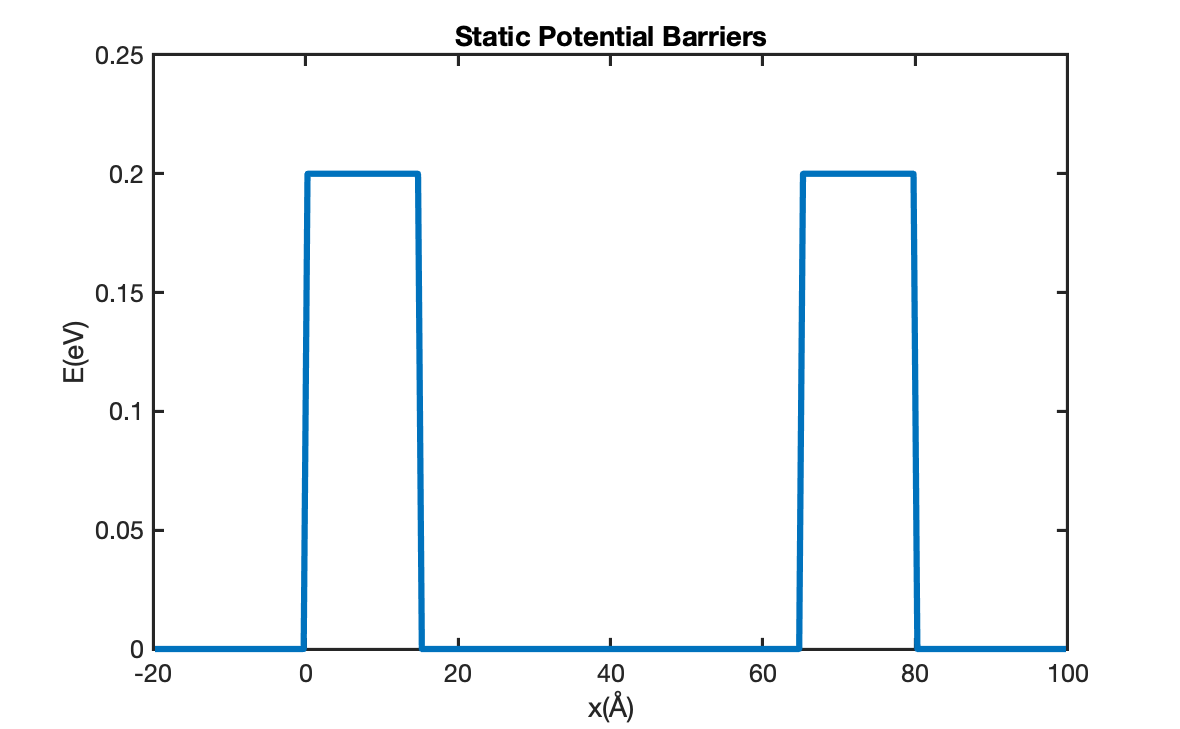
\includegraphics[width=0.9\linewidth]{Static_Potential_Barriers.png}
    \caption{Double potential barriers at 0.2 eV}
    \label{fig:example-1}
\end{figure}
Setting the step of the grid to $U(x)$ to 0.5 \AA. The lower bound $E_a$ is 0.0 eV and $E_b$ = 0.4 eV that are not affected by aliasing.

\begin{figure}[ht]
    \centering
    \hspace{-1cm}
    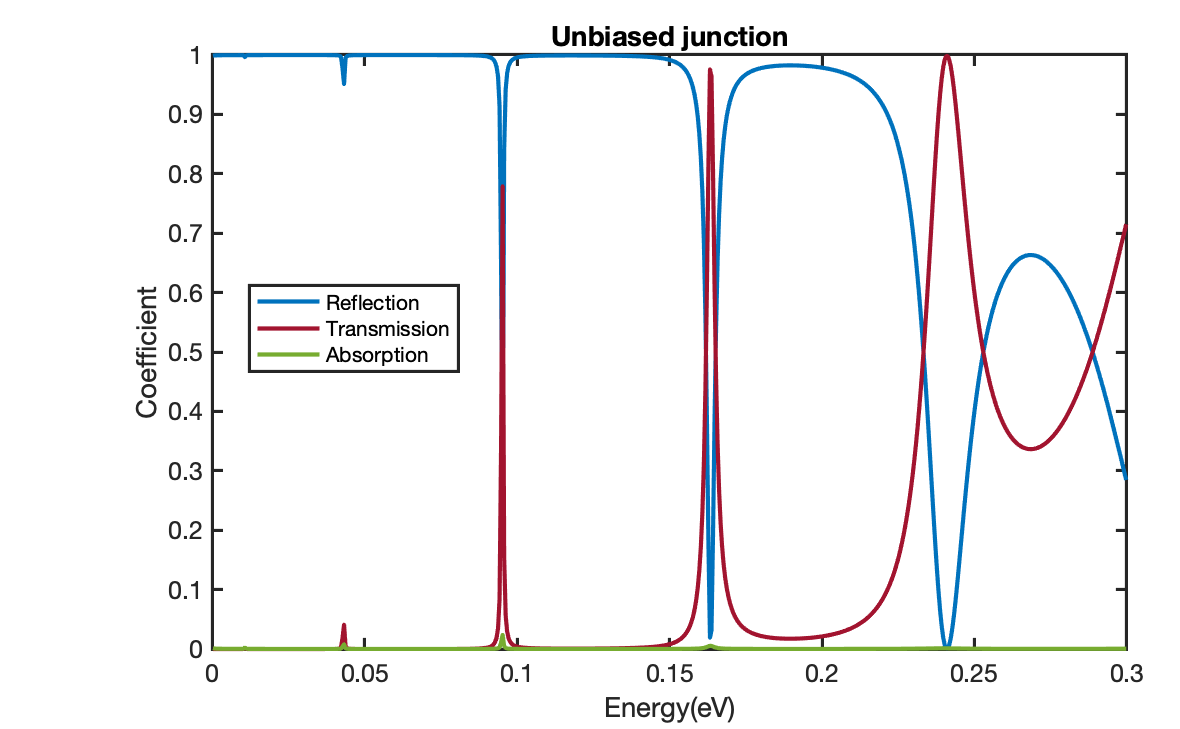
\includegraphics[width=0.9\linewidth]{unbiased_junction_spectra.png}
    \caption{Curves of the reflection, $R(E_0)$, transmission $T(E_0)$, and absorption coefficients $A(E_0)$ for $E_0$ $\in$ [0 eV, 0.3 eV] with steps as fine as 0.0005 eV, using a 1 nanosecond recombination time (lifetime) parameter.}
    \label{fig:example-2}
\end{figure}

After the potential barriers are defined, the curves of reflection, transmission, and absorption are calculated for $E_0$  [0 eV, 3 eV]. Figure 2. illustrates resonant tunneling with peaks in transmission at approximately 0.043 eV, 0.095 eV, and 0.163 eV, which align inversely with reflection dips, showing reduced reflection at these energies. Absorption is notably minimal, only slightly elevated at resonance points. All peaks are sharp suggesting a strong resonance effect at this energy level in the junction. Beyond 0.2 eV there is one more peak and dip at 0.23 eV, after transmission and reflection don't return to its initial coefficient, reflected by the fact that the barriers are 0.2 eV.
\begin{figure}[ht]
    \centering
    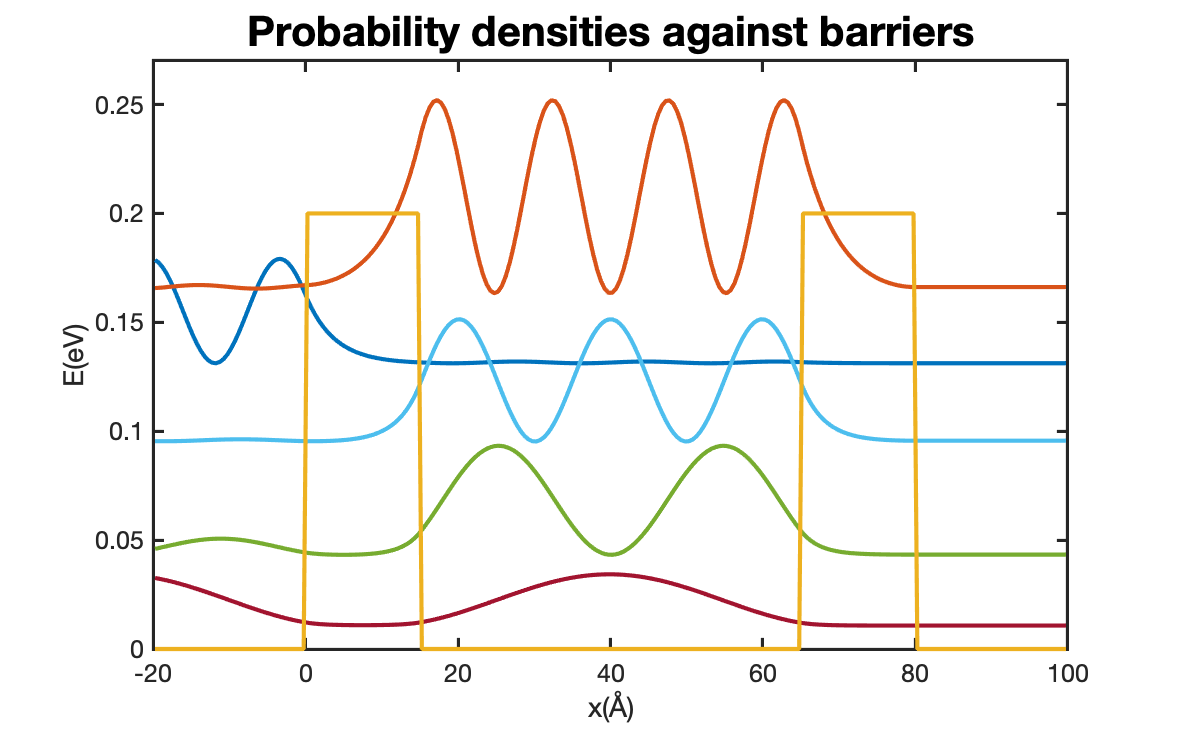
\includegraphics[width=0.9\linewidth]{prob_density.png}
    \caption{Quantum well probability densities show electron localization and energy quantization within potential barriers.}
    \label{fig:example-3}
\end{figure}

After identifying the energy levels at which transmission and reflection occur most significantly, the probability densities of the system are calculated. Figure 3. indicates that the energy level at which the probability of a particle tunneling through a potential barrier is significantly enhanced at the forementioned peaks. This occurs when the energy of the particle matches one of the natural frequencies of the system, allowing it to overcome the barrier with higher likelihood. The peaks in the transmission curve represent these resonant energies where the tunneling probability is maximized.

Regarding the reliability of the results, the peaks at 0.043 eV, 0.095 eV, and 0.163 eV are within the specified energy range [0.0, 0.4] eV. Given that they are between the lower limit \(E_a = 0.0\) eV and the upper limit \(E_b = 0.4\) eV, these resonances are considered reliable in the sense that they are within the expected energy window for this system. The peak at 0.1 eV is particularly significant since it is exactly at the midpoint of the specified energy range and may correspond to a fundamental resonance of the system.

The probability density graph correlates with the spectrum graph, where resonant peaks at around 0.043 eV, 0.095 eV, and 0.163 eV match energy states with 2, 3, and 4 peaks respectively, indicating increasing standing wave frequencies within the well. The highest number of peaks in the probability density reflects the highest resonance frequency. Conversely, the non-resonant state at 0.13 eV, with a flat probability density, aligns with minimal spectral features, denoting a lower frequency with no resonance. 

GaAs-AlGaAs heterostructures exhibit quantum resonance when electrons match the well's quantized energy levels, forming standing waves. Non-resonant states show no such alignment, hence no standing waves.

\begin{figure}[ht]
    \centering
    \hspace{-1cm}
    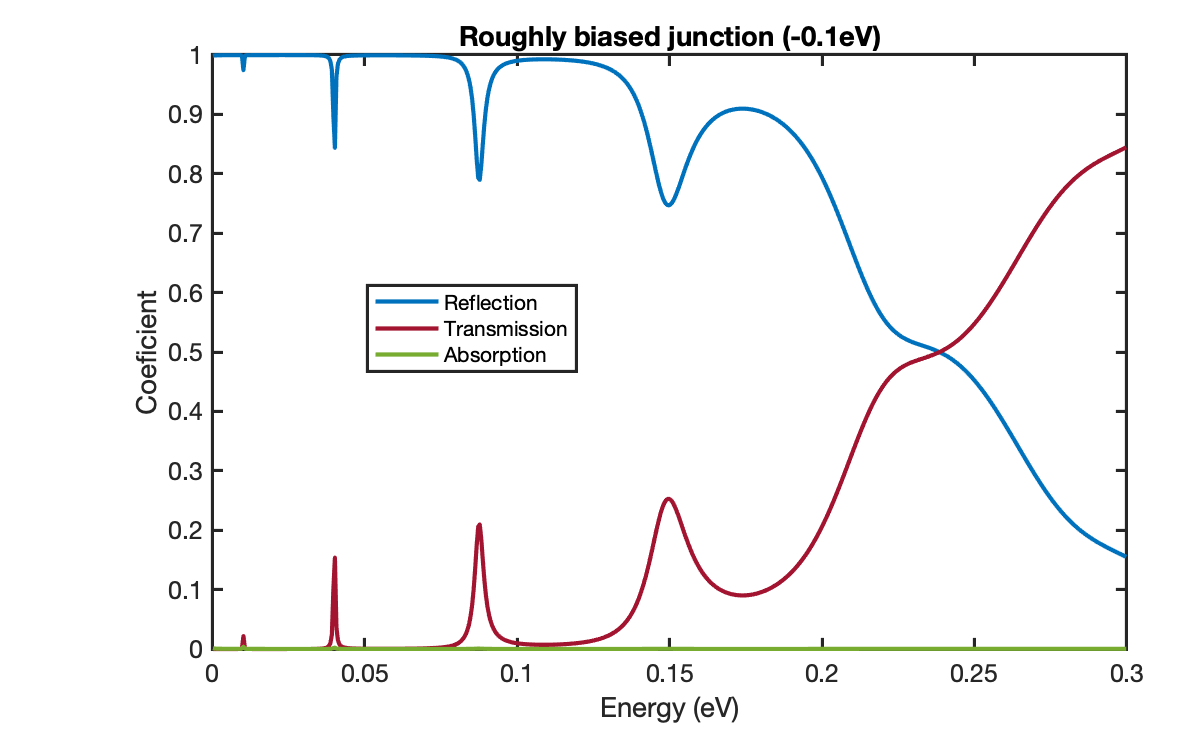
\includegraphics[width=0.9\linewidth]{roughly_biased_junction_spectra.png}
    \caption{Curves of the reflection, $R(E_0)$, transmission $T(E_0)$, and absorption coefficients $A(E_0)$ for $U(x') = 0.2 eV$ and $U(x') = 0.1 eV$.}
    \label{fig:example-4}
\end{figure}
In the biased junction spectrum, with barriers at 0.2 eV and 0.1 eV, transmission and reflection peaks are symmetrical yet less pronounced than in the unbiased case. This muted response is due to the lower energy of the second barrier, which smooths out the resonances, resulting in broader peaks and shallower dips at energies similar to the previous setup.
\subsection{Step function as reference system}

In the designated reference frame, the potential background is delineated by a step function: \( U_0(x < 0) = 0 \) and transitions to \( U_0(x > 0) = U_1 = -0.1 \) eV, indicative of a potential bias implemented across the junction. The Green's function, denoted as \( G_1(x, x'; k) \), adheres to the descriptions set forth in equations (A.76) and (A.77). Furthermore, waves impinging from \( x = -\infty \) and those transmitting towards \( x = +\infty \) are encapsulated by equation (A.65). This step function elucidates an electric field within the heterostructure, emanating from the stipulated potential bias.[1]

\begin{equation}
    G_{+,+}(x,x';z) = \frac{e^{iK_1 |x-x'|}}{2iK_1} + \frac{K_1 - K_0}{K_1 + K_0} \frac{e^{iK_2 |x+x'|}}{2iK_1}
\end{equation}

\begin{equation}
    G_{-,+}(x,x';z) = \frac{e^{-iK_0x + iK_1x'}}{i(K_0 + K_1)}
\end{equation}
    
\begin{equation}
    y_b(x) = e^{iK_0x} + r_b e^{-iK_0x}, y_b(x) = t_b e^{iK_1x}
\end{equation}
\begin{equation}
    |E| = -\frac{U_1}{x'_{\text{max}} - x'_{\text{min}}}
\end{equation}
\begin{equation}
    W(x') = U(x') - |E|x'
\end{equation}
\begin{figure}[ht]
    \centering
    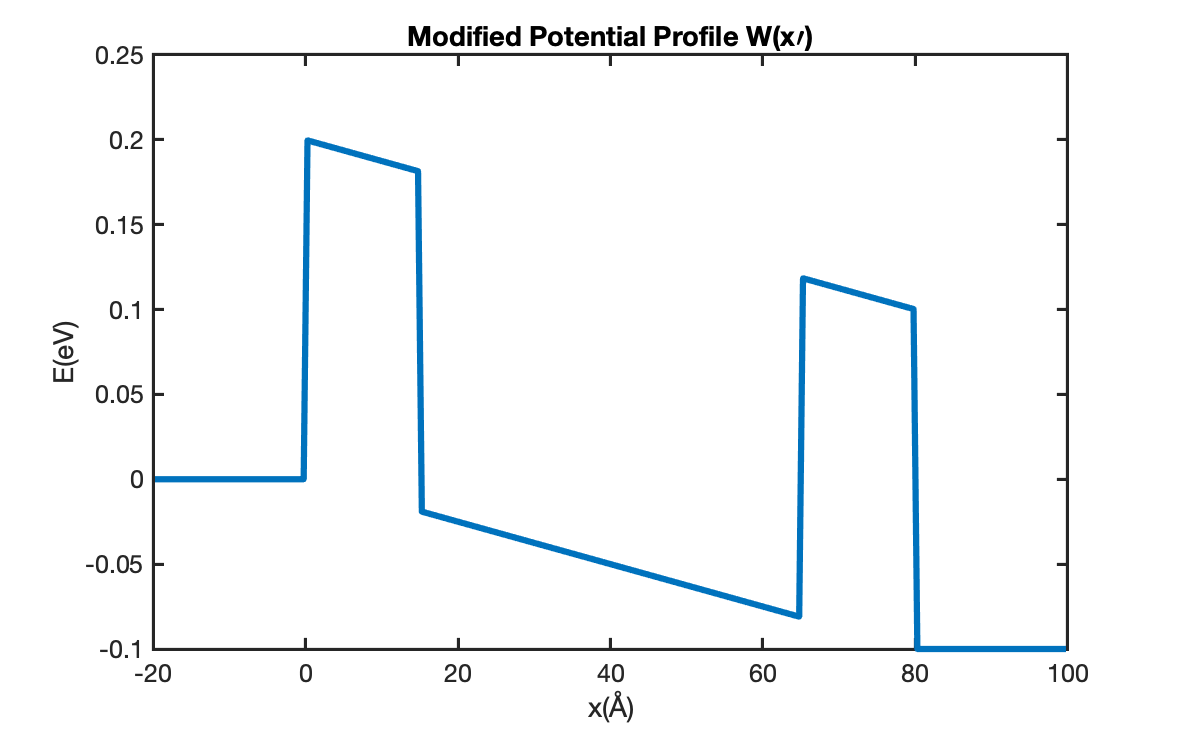
\includegraphics[width=0.9\linewidth]{biased_junction.png}
    \caption{Modified potential quantum well with E shifted down to -0.1 eV.}
    \label{fig:example-5}
\end{figure}
Given this, to avoid aliasing, $E_a$ and $E_b$ should be equals to -0.2 eV and 0.4 eV respectively.
\begin{figure}[ht]
    \centering
    \hspace{-1cm}
    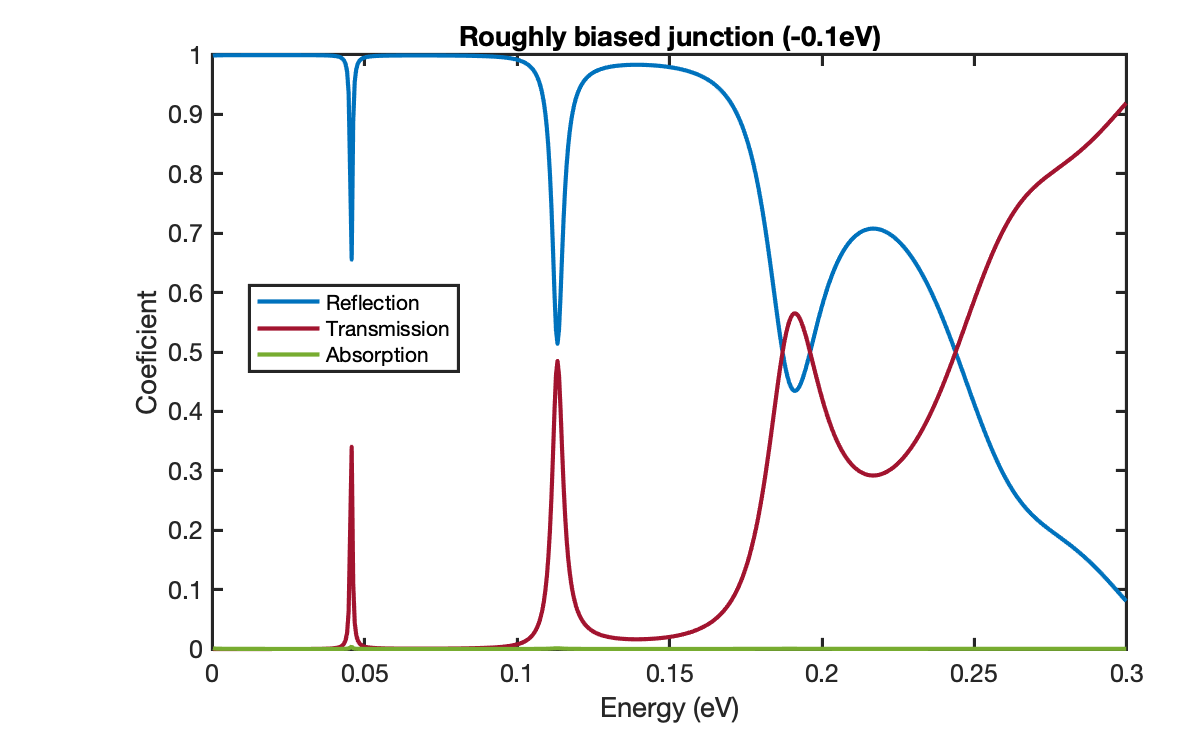
\includegraphics[width=0.9\linewidth]{roughly_biased_junction_spectra(-0.1eV).png}
    \caption{Spectrum of the modified well. The two visible transmission peaks at 0.04 eV and 0.11 eV}
    \label{fig:example-6}
\end{figure}
The biased junction's spectrum, influenced by a -0.1 eV bias, displays a sparser distribution of peaks in reflection and transmission, attributed to the second barrier's lowered potential. Notably, Figure 6. beyond 0.2 eV, the absence of pronounced peaks aligns with the diminished barrier height, altering the resonant conditions and reducing the likelihood of clear resonance formation, as the lowered barrier allows easier electron passage, thus smoothing out the spectral features.

\begin{figure}[ht]
    \centering
    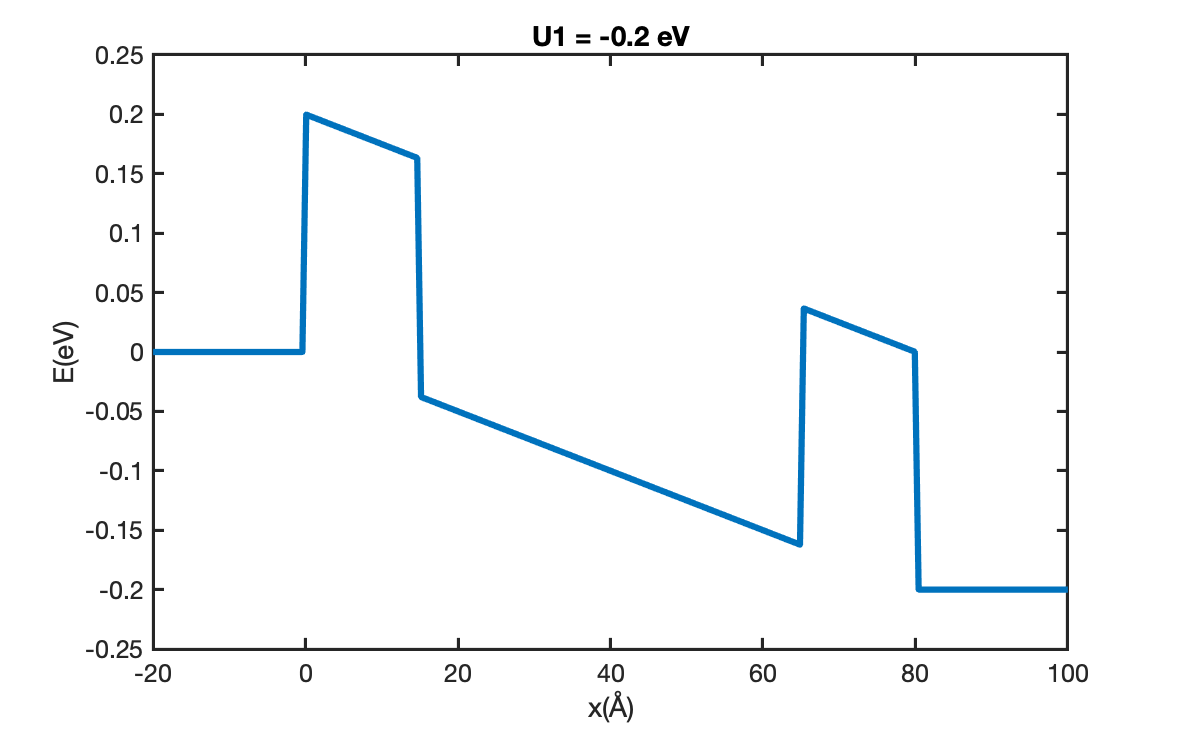
\includegraphics[width=0.9\linewidth]{U1_-0.2.png}
    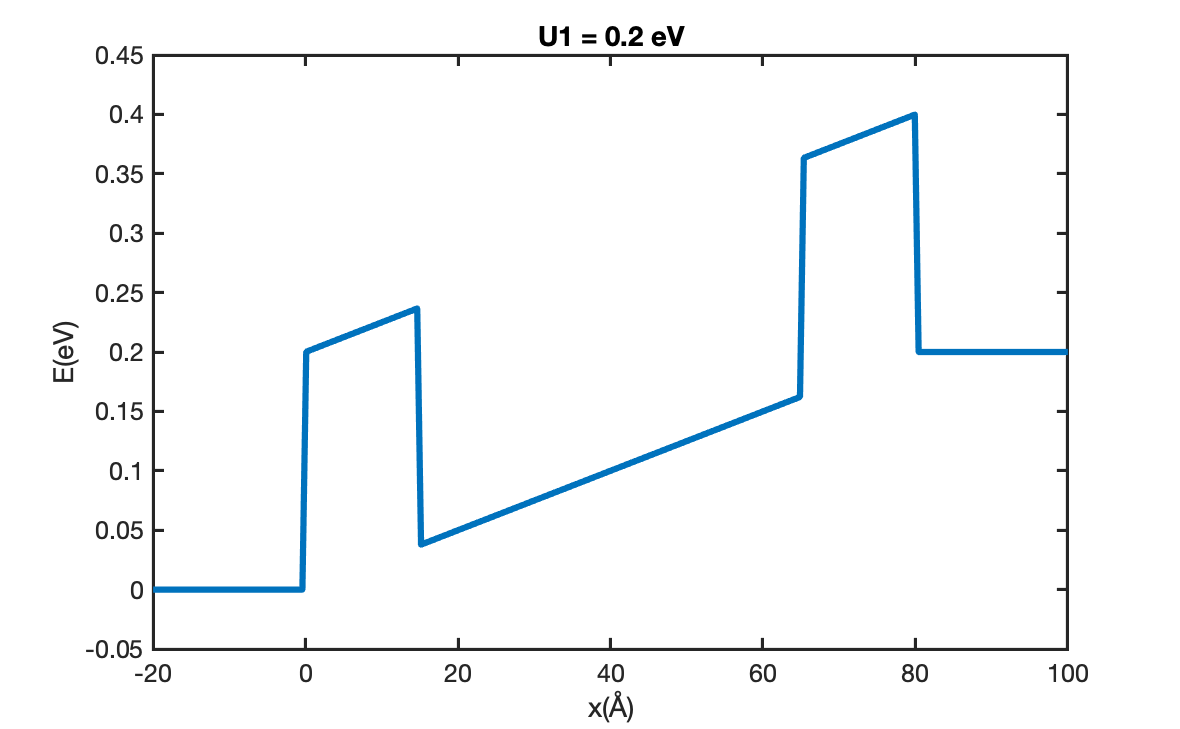
\includegraphics[width=0.9\linewidth]{U1_0.2.png}
    \caption{Bias adjustments in \( U_1 \) from -0.2 eV to +0.2 eV, considering both \( U_1 = -0.2 \) eV and \( U_1 = +0.2 \) eV.
    }
    \label{fig:example-8}
% \end{figure}

% \begin{figure}[ht]
    \centering
    \hspace{-1cm}
    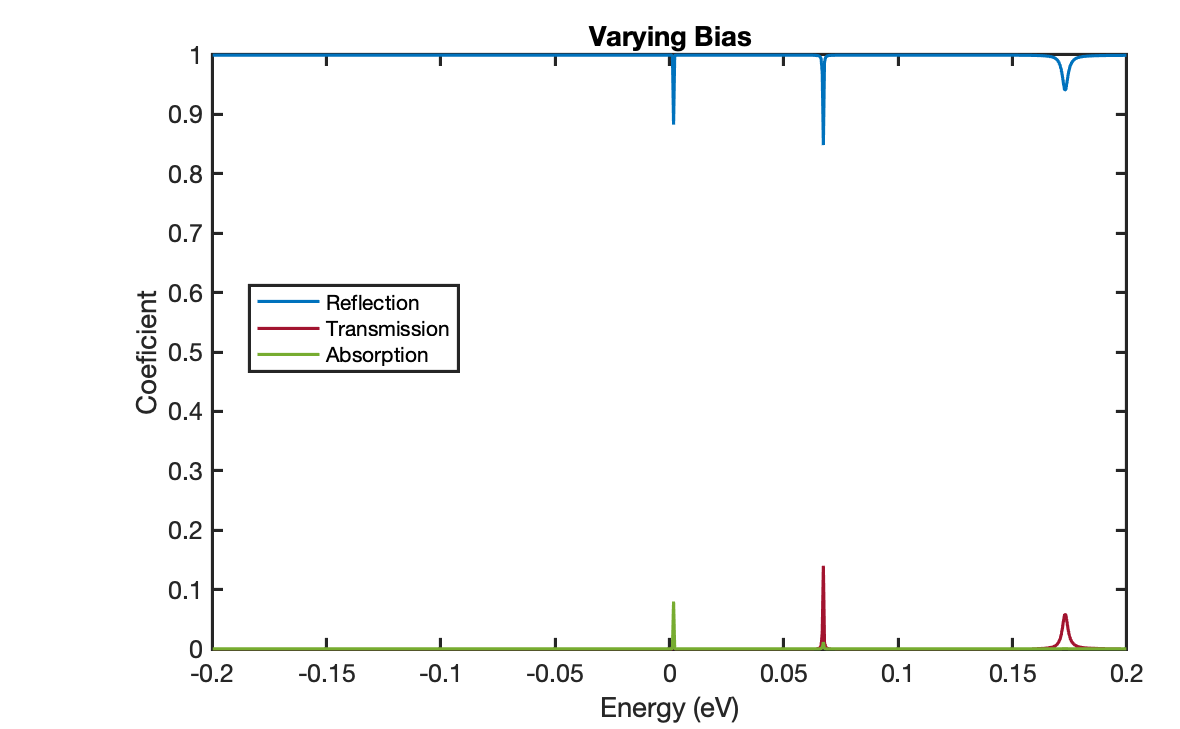
\includegraphics[width=0.9\linewidth]{varying_bias.png}
    \caption{Reflection and transmission flatline with peaks near 0.05 eV and 0.16 eV.}
    \label{fig:example-9}
\end{figure}

In the case of varying potential, the spectrum show a Negative Differential Resistence. The potential profiles for junctions biased at \(-0.2\) eV and \(0.2\) eV impact electron flow and resonance. For \(-0.2\) eV, the potential drop facilitates electron transition, as confirmed by the spectrum of varying bias, from -0.2 eV to 0 eV, no peak are observed. For \(0.2\) eV, the potential rise can hinder electron flow, enhancing NDR as transmission peaks sharply at resonance and then falls with increased misalignment of energy levels due to the bias.
The I-V curve derived from the spectral characteristics of the junction with varying bias is expected to display a non-linear behavior due to the quantum mechanical effects at play. Transmission shows moderate peaks at biases near 0.05 eV and 0.15 eV with coefficients peaking at 0.1 and 0.05, suggesting moderate increases in current at these energies due to resonant tunneling. Outside these peaks, the transmission remains low, and the reflection is high, indicating minimal current flow, leading to flat regions on the I-V curve. These features deviate from the linear response of an ohmic resistor and also from the exponential I-V characteristic of a diode. Instead, the I-V curve is anticipated to show distinct moderate peaks at certain biases and flat regions, underscoring the specialized behavior of the junction under the influence of the varying bias junction.

\section{Conclusion}
For the unbiased junction, the presence of distinct peaks in the transmission coefficient at certain energy levels indicated resonant tunneling, aligning with the quantized energy states of the quantum well. Probability density plots supported this, showing specific numbers of peaks within the well that corresponded to these resonant energies.

In the case of the roughly biased junction with a -0.1 eV bias, the spectral analysis revealed fewer and less pronounced peaks, suggesting that the lower second barrier affected the sharpness of resonant tunneling conditions. Despite the bias, the resonance energies appeared similar to the unbiased case, but with broadened features due to the modified potential conditions.

The varying bias spectrum showed evidence of Negative Differential Resistance (NDR), a non-linear phenomenon where increased bias leads to a reduction in current past certain resonant peaks. This behavior deviates from the ohmic response and is a hallmark of quantum devices that utilize resonant tunneling for high-speed applications.

\section{References}
[1]. Alain Dereux. Numerical Methods for Physicists. Universite de Bourgogne.

\end{document}
